\chapter{具体实现与实验步骤}
\label{chap:implementation}

在这个部分中,我们讲述详细的算法实现与实验步骤。
利用两组数据集,先生成满足条件的不完整信息网络,
然后使用距离学习算法学习距离。

\section{实验环境}

CPU:Intel(R) Xeor(R) CPU E7420 @ 2.13GHz

内存:64G

操作系统:Microsoft Windows Server 2003 Enterprise x64 Edition

其中采用Python语言实现DSHRINK算法和局部信息网络的生成以及一些自动处理的脚本,
Python的版本是Python2.7。使用Matlab完成DCA算法,PCA分析以及画出结果图,
MATLAB版本为MATLAB version 7.8.0(R2009 a) 64位版 。

\section{数据集的选取}
\label{sec:imple:dataset}

本文实验使用两组数据集,均来自于
\href{http://www.blogcatalog.com/}{Blogcatalog},
Blogcatalog是一个博客社交网络, 它把人们与博客作者及博客作者与博客作者联系起来,
从Blogcatalog的数据中,我们可以得到由用户组成的社交网络。
经过处理,我们得到了一个由88784个节点组成的社交网络,每一个节点拥有5413个特征属性。
有60个类作为Ground Truth验证最后的聚类结果,其中每个节点属于60个类中的一个或多个。

由于节点数目过多,所以通过取样的方式生成两组数据集,对于每一组数据集取样的方法如下:
首先从60个中选取6个包含1000个左右节点的类,然后选取属于这6个类中的所有节点作为当前的数据集中的节点。
通过这种方式,得到了数据集Blogcatalog-a和Blogcatalog-b,分别包含5118和5209个节点。

在选定了节点之后,需要对节点的属性进行处理,因为对于每一个节点,大部分属性值都是0,
这样的属性不适合用欧式距离或马氏距离作为节点之间的距离。所以采用PCA对节点的属性进行降唯,
最终选定了50个属性作为节点的属性。在使用PCA分析之前,必须对节点的属性正规化(Normalize)。

最终数据集的特征总结见表\ref{tab:datasetsummary}。

\begin{table}[!hpb]
  \centering
  \caption{实验采用数据集总结}
  \label{tab:datasetsummary}
  \begin{tabular}{rrrrr} \toprule
    数据集 & 节点数 & 边数  & 属性数 & 类个数\\ \midrule
    Blogcatalog-a & 5118 & 22863 & 50 & 6 \\
    Blogcatalog-b & 5118 & 25761  & 50 & 6 \\ \bottomrule
  \end{tabular}
\end{table}


\section{生成局部信息网络}

为了使用DCA距离学习算法,必须生成满足条件的不完全信息网络。
也就是说,必须要生成正语境限制和负语境限制。
本文生成正语境限制和负语境限制的方法如下:

为了生成正语境限制,必须找到相似集列表$C$,
需要在整个信息网络中取样一定数目的节点来生成$C$,
利用局部信息网络的特点,可以通过生成一定数量的特定大小的局部信息网络,
利用这些局部信息网络中的节点来生成$C$。定义局部信息网络的个数为regionNum,
局部信息网络的大小为regionSize。我们首先对节点按照与节点想关联的边的个数进行排序,
然后依次挑选一个节点作为一个局部信息网络的起始节点。对于第一个局部信息网络,
拥有边最多的节点被选中作为其实节点,然后利用宽度优先搜索(Broad First Search, BFS)添加节点到当前的局部信息网络,
直到regionSize个节点被添加。同样地,从排序的节点的列表中挑选边最多的未被访问的节点作为第二个局部信息网络的起始节点,
然后使用BFS添加节点,
依次类推直到生成regionNum个局部信息网络。利用这regionNum个局部信息网络所包含的节点来生成正语境限制。
对于任意两个节点,如果它们属于同样的类,那么它们就是相似的节点对,应该属于同样的相似集。
如果相似集$C_i$中的某个节点与相似集$C_j$相似,那么把$C_i$和$C_j$合并成一个相似集。

生成负语境限制的方法相对简单,只需要随机选取regionNum乘regionSize个节点用于生成负语境限制。
如果相似集$C_i$中的某个节点与相似集$C_j$不相似,那么$j \in D_i$且$i \in D_j$。

\section{结果好坏的评价标准}

为了评价本文提出算法的有效性,通过对比本文提出的算法和kmeans在Blogcatalog和
Blogcatalog-b上结果的好坏来判定。基于Ground Truth中包含的类的信息,我们使用聚类的纯度(Purity)来作为结果好坏的标准。
纯度的定义如下:

对于每一个聚类,在这个聚类中拥有最多节点个数的类作为这个聚类的标签,
属于这个标签的节点的个数是聚类的标签计数,
纯度等于所有聚类的标签计数和除以所有的节点个数。
数学表达为:

$$
Purity = \frac{1}{n} \sum_{i=1}^k \operatorname{max}_j |Cl_i \bigcap l_j|
$$

其中$\{C_1, ..., C_k\}$是所有的聚类,$\{l_1, ..., l_j\}$是所有的类。
根据定义可以知道,纯度越高,聚类的效果越好。


\section{实验结果}
\label{sec:results}

对于数据集Blogcatalog-a和Blogcatalog-b,
分别观察在不同的局部信息网络大小(一个局部信息网络中的节点个数)
和不同的局部信息网络的个数情况下的实验结果。
由于算法具有一定的随机性,对于每一种不同的情况,
重复实验5次,取平均值作为实验结果。

\subsection{不同的局部信息网络的大小}
\label{sec:results_node_max}

在Blogcatalog-a和Blogcatalog-b做社区挖掘所得到的纯度随局部信息网络大小不同的变化如图\ref{fig:node_max:a}。
此时选取的信息网络的个数为10。从实验结果可以看出,DSHRINK总是能比kmeans有更好的纯度,
同时总体的趋势是随着局部信息网络大小的增加,纯度变高。

\begin{figure}
    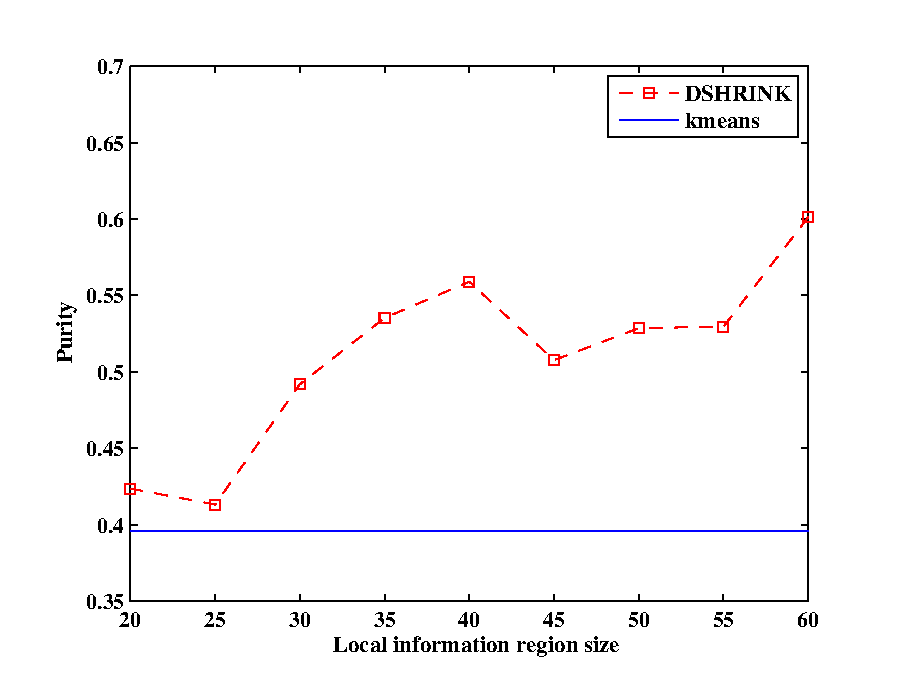
\includegraphics[width=1\textwidth]{chap2/blogcatalog_node_max}
    \caption{Blogcatalog-a在不同局部信息网络下的纯度}
    \label{fig:node_max:a}
\end{figure}

\begin{figure}
    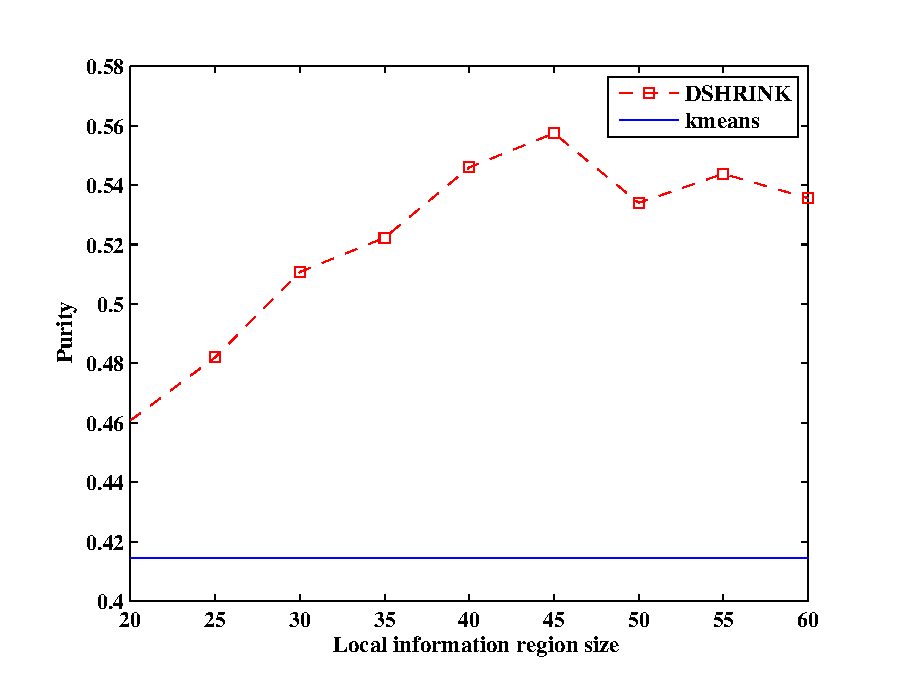
\includegraphics[width=1\textwidth]{chap2/blogcatalog_b_node_max}
    \caption{Blogcatalog-a在不同局部信息网络下的纯度}
    \label{fig:node_max:a}
\end{figure}

%\begin{figure}
  %\centering
  %\subfigure[Blogcatalog-a]{
    %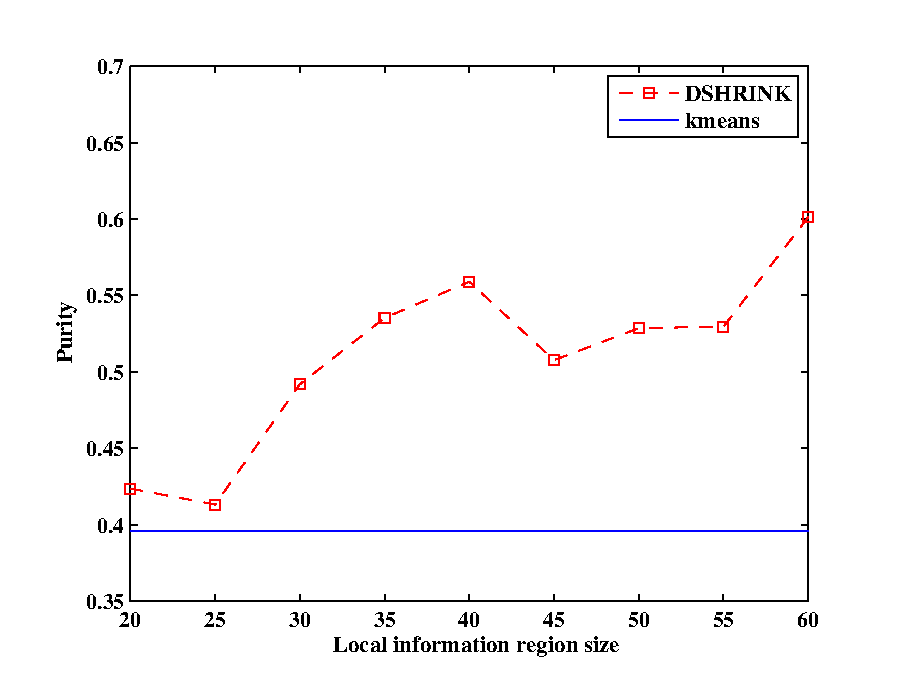
\includegraphics[width=0.45\textwidth]{chap2/blogcatalog_node_max}
    %\label{fig:node_max:a} %% label for first subfigure
    %}
  %\subfigure[Blogcatalog-b]{
    %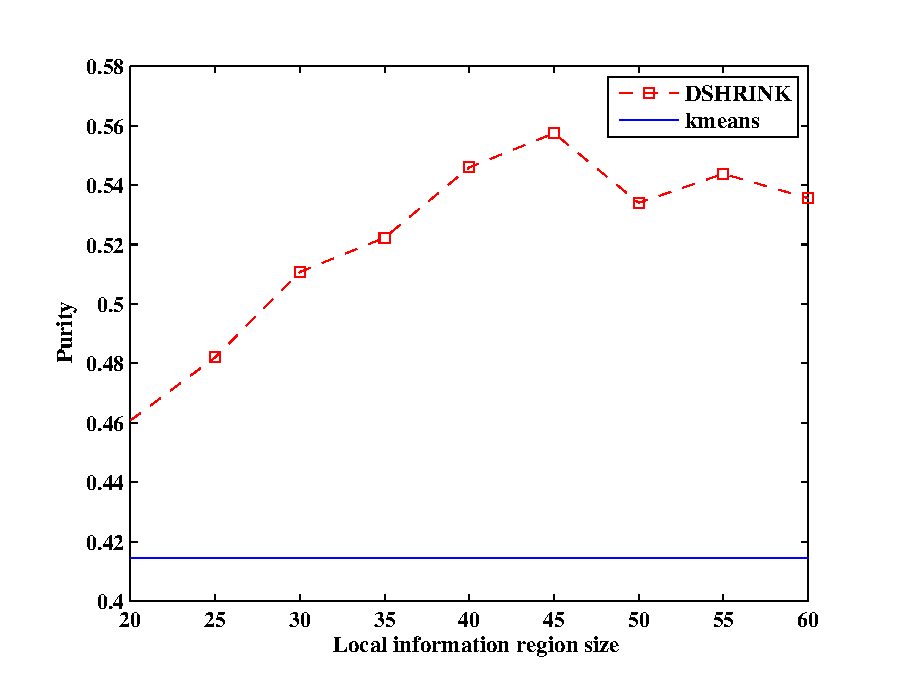
\includegraphics[width=0.45\textwidth]{chap2/blogcatalog_b_node_max}
    %\label{fig:node_max:b} %% label for second subfigure
    %}
    %\bicaption[fig:node_max]{不同局部信息网络大小下的纯度}{不同局部信息网络大小下的纯度(信息网络个数为10)}{Fig}{Purity under different local region information size}
%\end{figure}

\subsection{不同的局部信息网络个数}
\label{sec:results_region_num}

在Blogcatalog-a和Blogcatalog-b做社区挖掘所得到的纯度随局部信息网络大小不同的变化如图\ref{fig:region_num}。
此时选取的信息网络的大小为50。从实验结果可以看出,DSHRINK总是能比kmeans有更好的纯度,
同时总体的趋势是随着局部信息网络大小的增加,纯度变高。

\begin{figure}
  \centering
  \subfigure[Blogcatalog-a]{
    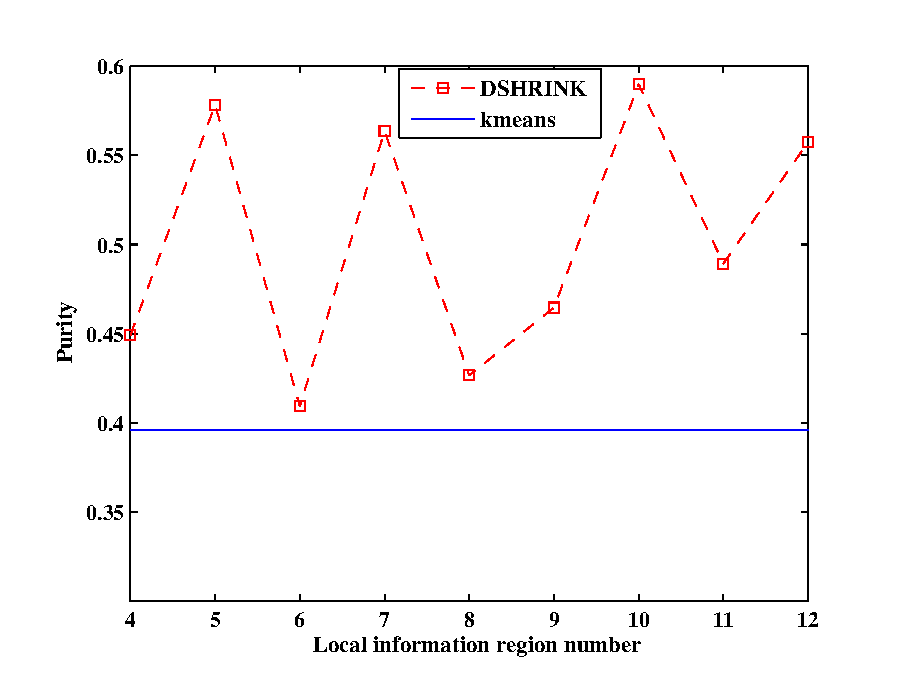
\includegraphics[width=0.45\textwidth]{chap2/blogcatalog_region_num}
    \label{fig:region_num:a} %% label for first subfigure
    }
  \subfigure[Blogcatalog-b]{
    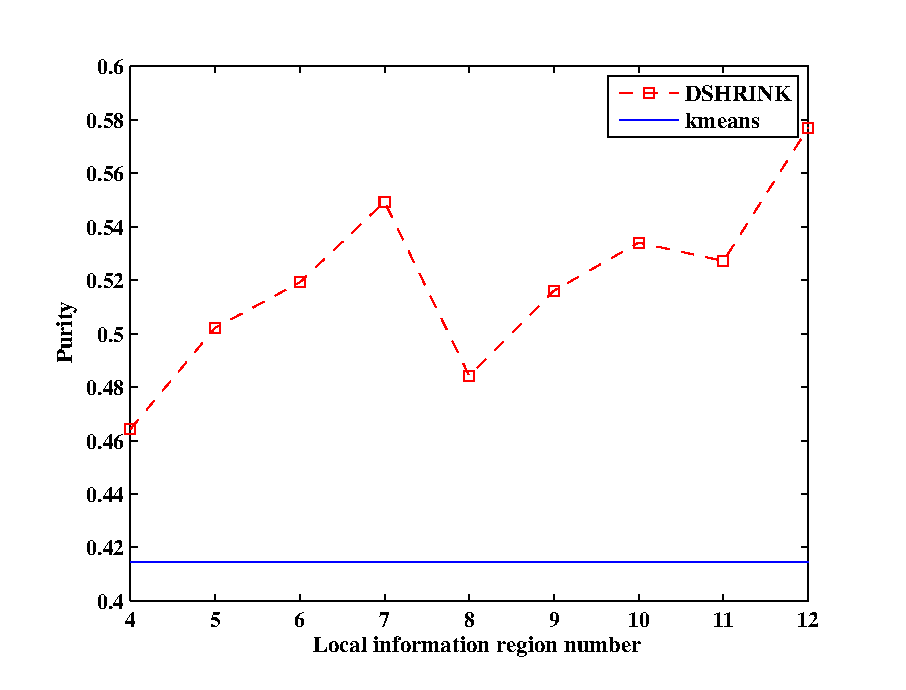
\includegraphics[width=0.45\textwidth]{chap2/blogcatalog_b_region_num}
    \label{fig:region_num:b} %% label for second subfigure
    }
    \bicaption[fig:region_num]{不同局部信息网络个数下的纯度}{不同局部信息网络个数下的纯度(信息网络大小为50)}{Fig}{Purity under different local region information number}
\end{figure}

\subsection{实验结果分析}

DSHRINK相对于kmeans有更高的纯度是因为kmeans只是单纯地根据节点之间的欧式距离进行聚类,
而DSHRINK根据已知的信息在欧式距离的基础上进行了一定的调整,能够达到更好的聚类效果。
而且,知道的信息越多,纯度越高。

